\documentclass[letterpaper, 10pt,titlepage]{article}

\usepackage[utf8]{inputenc}
\usepackage [english]{babel}
\usepackage{graphicx}
\graphicspath{}
\newcommand\tab[1][1cm]{\hspace*{#1}}
\setlength{\parindent}{0em}
\setlength{\parskip}{1em}
\usepackage[letterpaper, margin=0.75in]{geometry}
\usepackage{balance}
\usepackage{hyperref}
\usepackage{minted}
\hypersetup{
  colorlinks = true,
  linkcolor  = black
}

\setcounter{secnumdepth}{4}
\def\name{Group 48}

\graphicspath{ {images/}}

\hypersetup{
  colorlinks = true,
  urlcolor = black,
  pdfauthor = {\name},
  pdfkeywords = {Winter Midterm Progress Report},
  pdftitle = {Capstone Project},
  pdfsubject = {Capstone Project},
  pdfpagemode = UseNone
}



\begin{document}

\begin{titlepage}
\begin{center}
    \Huge
    \textbf{Winter Midterm Progress Report}
    \textbf{Capstone Project}\\
    \vspace{1.0cm}
    \large
    Developers: Sung Kim, Xiaoli Sun, Zijian Huang\\
    Client: David Vasquez\\
    \vspace{1.5cm}
    \large
    Instructor: D. Kevin McGrath\\

    \large
    CS 462, Winter 2018, Oregon State University\\    

    \vspace{3.2cm}

    \large
    \underline{Abstract}\\
    \vspace{0.3cm}
    \end{center}
    \large

    \tab For the Campus Event Mobile Application program, the client David Vasquez want to make life more convenient for each students, instructors or even residents live in Corvallis since there are lots of events happen everyday. A great mobile application is useful for every user and improve the quality of life. The mobile application will be developed in two forms: one developed for the Android mobile platform, and the other developed for the iOS mobile development. For the ease of development, these two forms of the mobile application will be developed with a framework called React Native which support cross platform development, they will be using the same methods of providing campus events to users. The mobile application will display current events and group events by loading data from MySQL database. In addition, the mobile application will allow users discover different events from different sections, follow and unfollow events, and edit user profile. 
    \vspace{0.8cm}
    \vfill
    
\begin{center}    
    Feb 15, 2018

\end{center}
\end{titlepage}


\tableofcontents
\newpage

\section{Introduction}
Various organization holds multiple events every year in Oregon State University. To let the Corvallis community more involved, Evently will display multiple group events to the public. The mobile application will provide user interact calendar as a view to keep track of all the events that they want to see. Users will also available to find new events according to different categories. Moreover, users have access to discover all groups that they interested and can participate with. The mobile application will have secure login to further protect user information. The application is developed under React Native. 


\section{Xiaoli Sun's section}
\subsection{Current status}
Currently, I am working on the user interface of the mobile application. As I introduced above, the application contains 4 main screens: Events, Discover, Following and Profile. Three screens will be embedded in the Events screen to show contents in different views including calendar view, list view and box view. First, I created a new folder called src in root directory of the mobile application. Inside this folder, I created couple sub folders to store files for different screens. After that, I created a file called index.js. In this file, I made a tab navigator with footerbar which holds the 4 main screens: Events, Discover, Following and Profile. Most of time that I spent on this screen was to find how to change the background color of footerbar and add icons. In Events screen, I created a tab navigator to hold three screens which are used to display contents in different view. A stack navigator was also created to hold the tab navigator to let the screen to be displayed at the top. In Discover screen, I made 4 touchableOpacity objects with images to represent different categories of events. Currently once user click the button, only a dialogue box will be pop up. In Following screen, I only added some dummy data inside this screen. 

\subsection{What's left}
A lot of work are needed to be done in application development. The most complicated work that I think is how to implement oAuth 2 in the mobile application. I made many researches on Internet to find out how oAuth 2 works and how to implement oAuth 2 to project. However most of the tutorials of oAuth 2 for React Native is all based on social media like Facebook, Google, Twitter, Instagram and so on. Most of these social media platforms provide developing kit and packages to developers for the ease of development. However, OSU don’t provide such packages for developers, thus I have implement oAuth 2.0 totally by myself. Because the oAuth 2.0 that will be used in our mobile application is provided by OSU, which means the application will use deep linking API to open a OSU authentication web page in the in-app web browser, once user’s authentication is approved, he will be redirected to our application. I will keep working on how to implement oAuth 2 in our application. The second work that I will implement is to link the mobile application to MySQL database to retrieve events data. I totally have no experiences on linking React Native application to database but I will try my hard to achieve this target. 

\subsection{Issues}
During the development of using React Native, the major problem is that the only experience that I have for JavaScript development is in CS 290 class. Although I took CS 496 (Android mobile application development) before, developing in React Native is totally different than Android. Moreover, because React Native is a pretty new framework, some wired problems could be found during development. The second problem that spent me a lot of time to fix was how to customize theme to footerbar which was created in index.js. The last problem is that testing iOS version of the application is hard for me to implement. Android version of the mobile application can only be tested in Android emulator and iOS version can only be tested in macOS. However, I only have a PC thus I can only test whether the mobile application works under Android or not.

\subsection{Solutions}
To have a first and quick impression of how to implement application using JavaScript, I made a lot of researches about React Native on Internet before implementing the project. The first thing that I looked over was React Native documentation. React Native documentation provides basic installing set up tutorial, tons of APIs and brief description and codes of these APIs to developers. I followed the tutorial in the documentation to create a new project and learned how basic components are created by using React Native. After an empty project was created, I searched online to find out how to handle navigation in React Native, fortunately I found two packages: React Navigation and Native Base. A full example of React Navigation can be found at Native Base website which gave me a lot of help. After reading documentation of Native Base, I found a way to customize themes for footerbar which means I can add icons and change background color of footerbar. A wired problem was occurred during implementing tab navigator in Events screen. The content couldn’t be displayed correctly on tab navigator in Events screen. After spending long time online searching for solution, I finally fixed this problem. The solution was simply to change both animationEnabled and swipeEnabled to false. The last problem could be fixed by using Zijian’s MacBook for testing iOS version of application. 

\subsection{Other Information}
The interesting piece of code is index.js. In this file, I used getTheme and material to customize themes for footerbar rather than creating a stylesheet directly in this file because stylesheet didn’t work for customize footerbar.

\subsection{JavaScript code for homescreen}
\begin{minted}{javascript}
import React, { Component } from "react";
import Events from "./Events.js";
import Discover from "./Discover.js";
import Following from "./Following.js"

import getTheme from 'CampusEventApp/native-base-theme/components';
import material from 'CampusEventApp/native-base-theme/variables/material';
import { TabNavigator, DrawerNavigator } from "react-navigation";
import {
  Button,
  Text,
  Icon,
  Item,
  Footer,
  FooterTab,
  Label,
  StyleProvider
} from "native-base";
const HomeScreen = TabNavigator(
  {
    Events: { screen: Events },
    Discover: { screen: Discover },
    Following: { screen: Following }
    //Profile: { screen: Profile}
  },
  {
    tabBarPosition: "bottom",
    tabBarComponent: props => {
      return (
        <StyleProvider style={getTheme(material)}>
        <Footer>
          <FooterTab>
            <Button
              vertical
              active={props.navigationState.index === 0}
              onPress={() => props.navigation.navigate("Events")}
            >
              <Icon name="globe" />
              <Text>Events</Text>
            </Button>
            <Button
              vertical
              active={props.navigationState.index === 1}
              onPress={() => props.navigation.navigate("Discover")}
            >
              <Icon ios="ios-paper" android="md-paper" />
              <Text>Discover</Text>
            </Button>
            <Button
              vertical
              active={props.navigationState.index === 2}
              onPress={() => props.navigation.navigate("Following")}
            >
              <Icon ios="ios-add-circle" android="md-add-circle" />
              <Text>Following</Text>
            </Button>
             <Button
              vertical
              active={props.navigationState.index === 3}
              onPress={() => props.navigation.navigate("")}
            >
              <Icon ios="ios-person" android="md-person" />
              <Text>Profile</Text>
            </Button>
          </FooterTab>
        </Footer>
        </StyleProvider>
      );
    }
  }
);

export default HomeScreen;

\end{minted}


\section{Sung Kim's section}
\subsection{Current Status}
One of the key components of this application is having the ability to hold various amounts of data in a secure location. We decided to use a relational database to hold all of our information. MySQL helps us manage that database by giving us the ability to easily manipulate it as we see fit. Plus, the knowledge I gained from my previous internship allowed for me to jump right into managing our data.

For the current status of my work, I am creating the tables that will hold all of our information. Our application needs multiple tables connected by various primary keys depending on the user. Our client, David Vasquez, also had knowledge of managing these databases and provided me with some tables that he would like for me to review. I am currently looking at the structure of these tables to see if they have been normalized or not. Table normalization is key for designing any database; this lets tables be less cluttered with large amounts of information and allows for faster search. Another way to speed up searching through these tables is by adding indexes. Indexes allow us to find rows with specific columns values quickly. These are especially useful for larger tables, because it gives us a starting place to look instead of having to search through the entire table looking for one entity. To manage and look at our current tables, David has also recommended me a tool to easily manage this. The tool WampServer is essentially a bundle of software you can use to manage multiple development tools for a database. It consists of OpenSSL, an Apache web server, MySQL database and support for the PHP programming language. With this tool, we can create our local servers and start testing our mobile app with data we provide. So far, development is moving along nicely and is currently starting to show some results.

\subsection{What's left}

As for what’s left to do on my side of development, I currently need to fill our database with some information. We currently have no “real” event data we are working with, so as a temporary solution I will be adding some fake data to test if our application can display the information properly. There are more details about this issue in the next section of this report. As for the group, we still have a lot left to do. Starting with things such as completing the user interface and connecting our database to the actual application. After completing these two tasks we will move on to implementing oAuth 2.0 and finding a place to host all of our data. I will start by adding the list view for events to our application to easily see the information. This will be done before attempting to put information on the calendar to make sure we are getting the right data. Although some of the new tools we are using started off as being completely foreign to us, we can finally start a small conversation about these tools. In our meeting with David Vasquez on Feb. 12, he was pleased with the current look of the application.

\subsection{Issues}

Some current issues we are facing with our application include receiving “real” data from various groups in our community. Xiaoli has reached out to OSU asking for a possible API we could use to grab data from the OSU events calendar. Unfortunately they did not have one. For a temporary solution to this issue we have decided to manually throw in some data into the tables. Another possible solution includes adding an admin functionality for event hosts to manage and apply certain changes for themselves. Another issue we are currently running into is not having a centralized database to retrieve the information from. Currently, this is not a big issue, since we still need to connect our database to the application, but will pose problems in the future. This issue has been brought up with David and he is looking into some solutions for a remote server. As of now, we are using local databases on our machines and creating identical the tables using the same SQL code. This will let our code have some uniformity when retrieving data from our future remote server.

\subsection{Other Information}

Some other relevant and/or interesting pieces of information include David asking us to continue working with him on this application. Once we have finished our work for this class, David wants to see how popular this application will be. He is probably one of the coolest guys I have worked with and the fact that he is truly passionate about this application motivates me more to deliver a quality product. Also React Native is a very interesting tool that we are using for the development of this application. Being able to test our work on our actual phones, using the Expo app, truly let’s us see how it will look and feel for our users. What’s even greater than that is being able to see it work on both Zijian’s iPhone and my Android. There were some bumps along the way that slowed the development of the application, such as Xcode not cooperating with us in the beginning, but that problem is long gone.

\section{Zijian Huang's section}
\subsection{Current Progress and Issues}
I am taking part of IOS platform application development. In IOS, our team also choose React Native to develop mobile application in IOS platform. The difficulty is I have no experience to developing with React Native, so I didn't know how to set up for React Native in macOS platform for developing IOS on Xcode. Xcode as we know is the most useful developing IDE on macOS and it is the best developing IDE for IOS developer. Setting up the new items is always difficult, and I am learning how to set the React Native works on Xcode. When I am worrying about how to do that, fortunately, team member Xiaoli has already made a Android platform sample for testing, and he allowed me to test on macOS to see if we can show up on IOS simulator, Expo app, it works. Right now I should to discuss with Xiaoli about the development since the programming of this development should work both IOS and Android platforms right now. While the condition allows, Xiaoli and I will develop this application together.

\subsection{What's Left}
Right now, I am working on setting up the React Native and hope it could be finished earlier, then I will focusing on IOS developing, include the functionalities which we plan to do in our application, connecting data to database, and fix bugs. Also, our client David wants to add the QR code scan function in our application as an additional option. I do some research on the scan function in React Native and there are some samples, so in the developing part, it is not a very big challenge for us. But to using this scan function to read QR code during big event like football game or by using scan QR code to give users bonus in the campus are the most difficult thing because we have no resource to get permission. For the most of IOS platform developing, the goal is the application will have the same functionality as Android platform and the interface will looks like as same as Android platform. When user get this application and own their personal account, we hope there will have no bugs or crush come out. Be perfect is the first purpose of us, and we really want to develop a great application for our Corvallis community.

Also, our team have the plan for develop a website page as the browser platform or an official web page for our Evently mobile application. For this part, I am using the CS290 and CS340 classes as the foundation since HTML, CSS, JavaScript and PHP are learned from these two classes. Also, for the database, SQL is an option for us in the data storage part. The plan for this web page is an additional option for our team, if the development progress well and our team have enough time available, we will make the browser platform as wish because we want to be more profession and better on this application development. Recent plan for this web develop is I am preparing the front-end development, include HTML, CSS and little of JavaScript. Hopefully the front-end development will be delivered around the beginning of the next term for backup. At that time, if there have many things happened during the mobile application development, team should focusing on that problems rather than create a new platform, then the front-end development backup will be abandoned since our client David not require us to take risks doing a new platform. 

\subsection{Other information}
For this application, all the team members want to present the best version and our client David gives us lots of advises and encourages. Everyone in this team want to bring new features as soon as possible because we really want to do something which could help others in the future who lives in Corvallis. The reason why we work hard is because David said he wants to see how popular this application will be and if the application get popular when it come out in OSU or even in Corvallis community, he will make it like a formal version of application, which means the app will continue be updates and try to let more people who lives near Corvallis or not to use it. At that time, we will be proud since we are the founding members of this app. So for this app, we have a lot of new idea come out everyday since we want to give this app more functional features, when people use it, the features could really helping them to make convenient. That is the original goal for all the teammates.

\section{Conclusion}
Overall the progress of this project is moving along smoothly. While there is still a lot left to do, our progress is starting to show some results. The user interface is coming along nicely, we will soon be ready to connect our application to the database, and  there is functionality for both Android and IOS.

\section{Screenshots}
Campus Event Mobile Application which developed by Group 48 shows the design viewpoint above. Each of the features will suitable for every requirements for this mobile application. Also, the design must be clearly and usefully since our group is going to focus on develop this whole application step by step and make sure we are efficient and try to make no mistakes during developing. 
\newpage
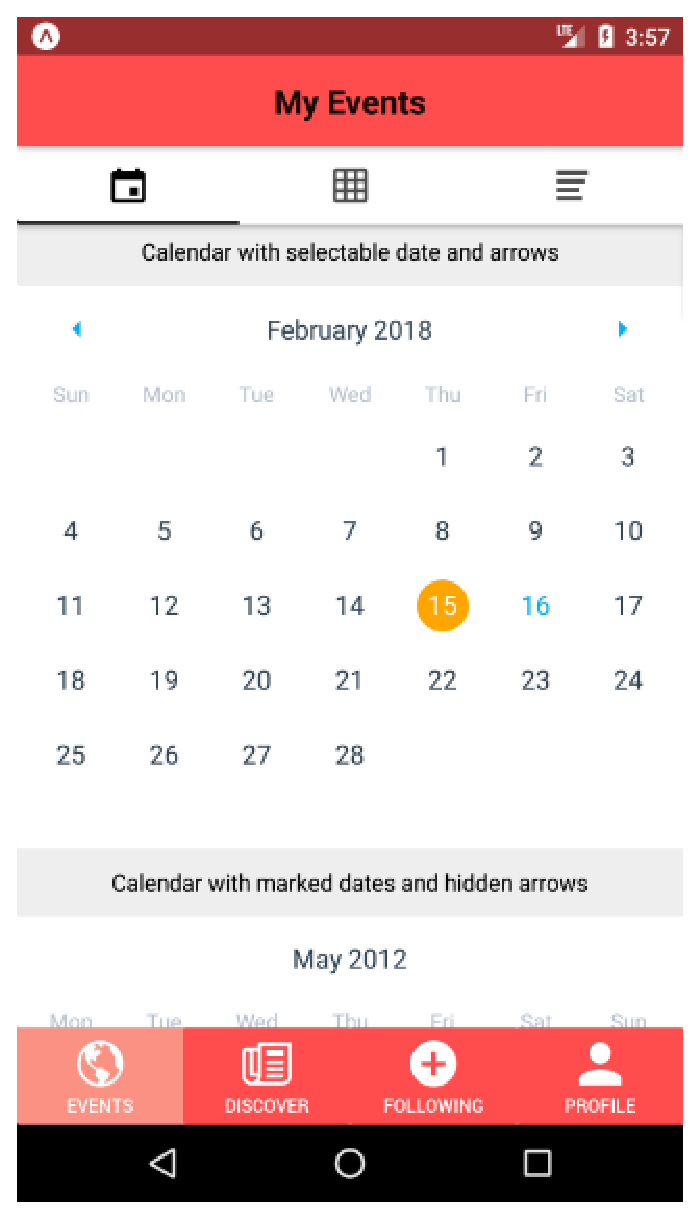
\includegraphics{Calendar_View.eps}
\newpage
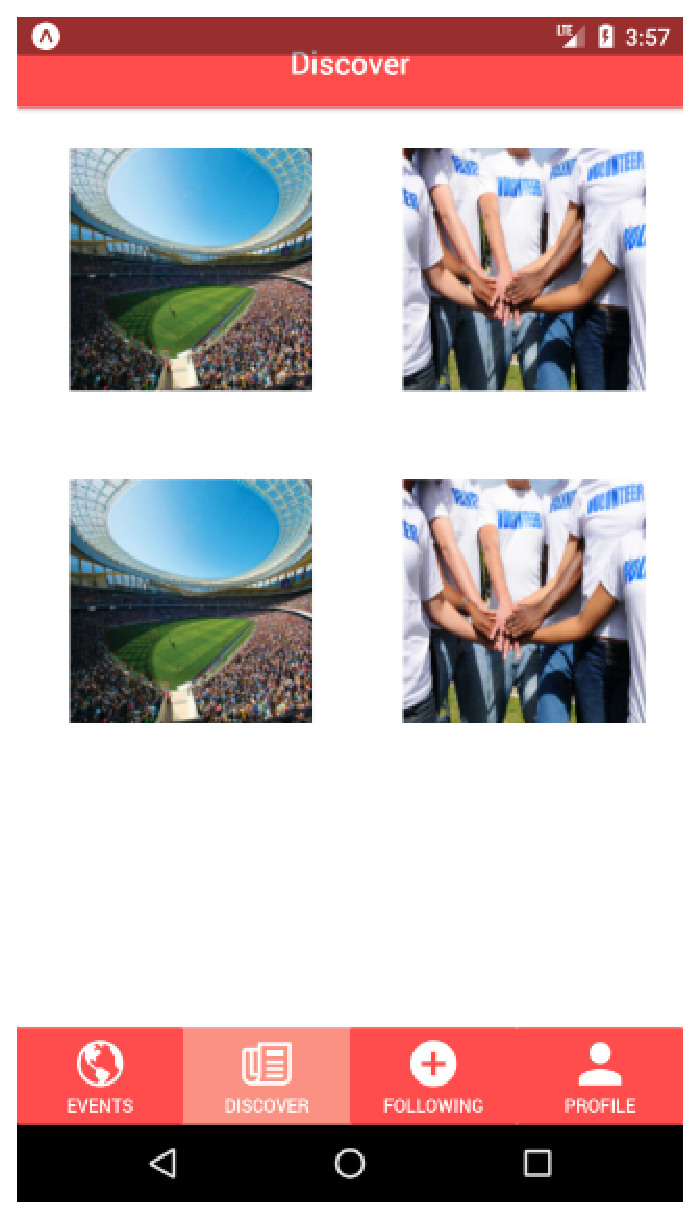
\includegraphics{Discover_Screen.eps}
\newpage
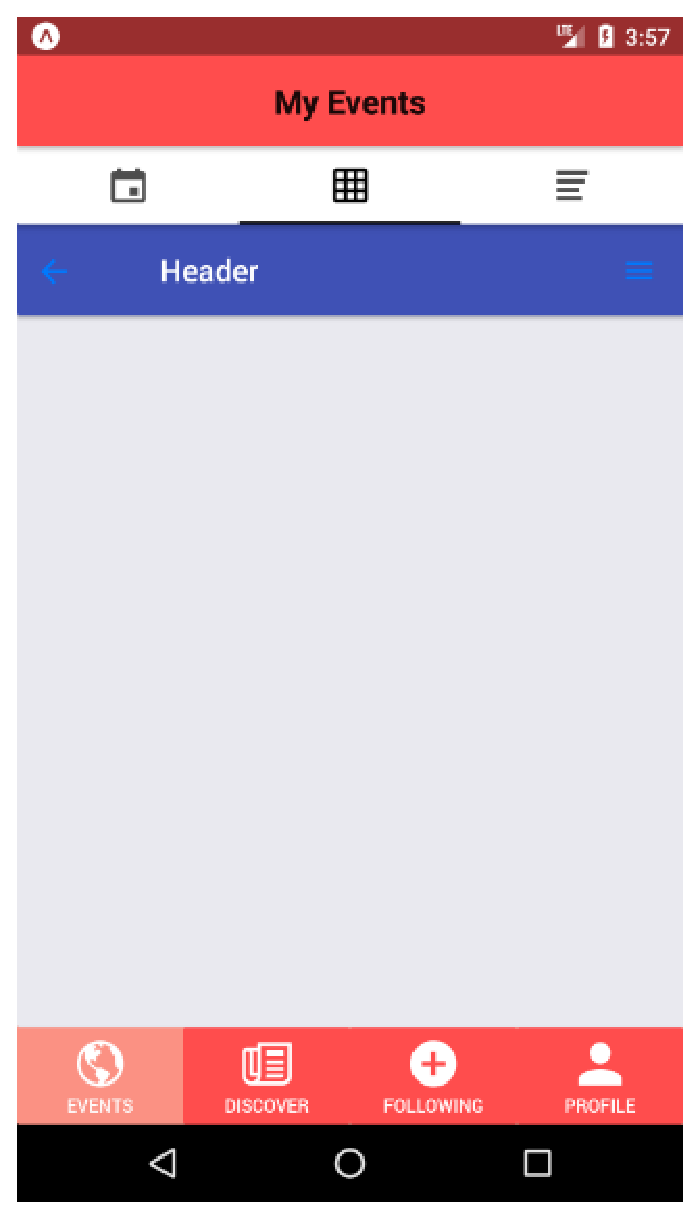
\includegraphics{Box_View.eps}
\newpage
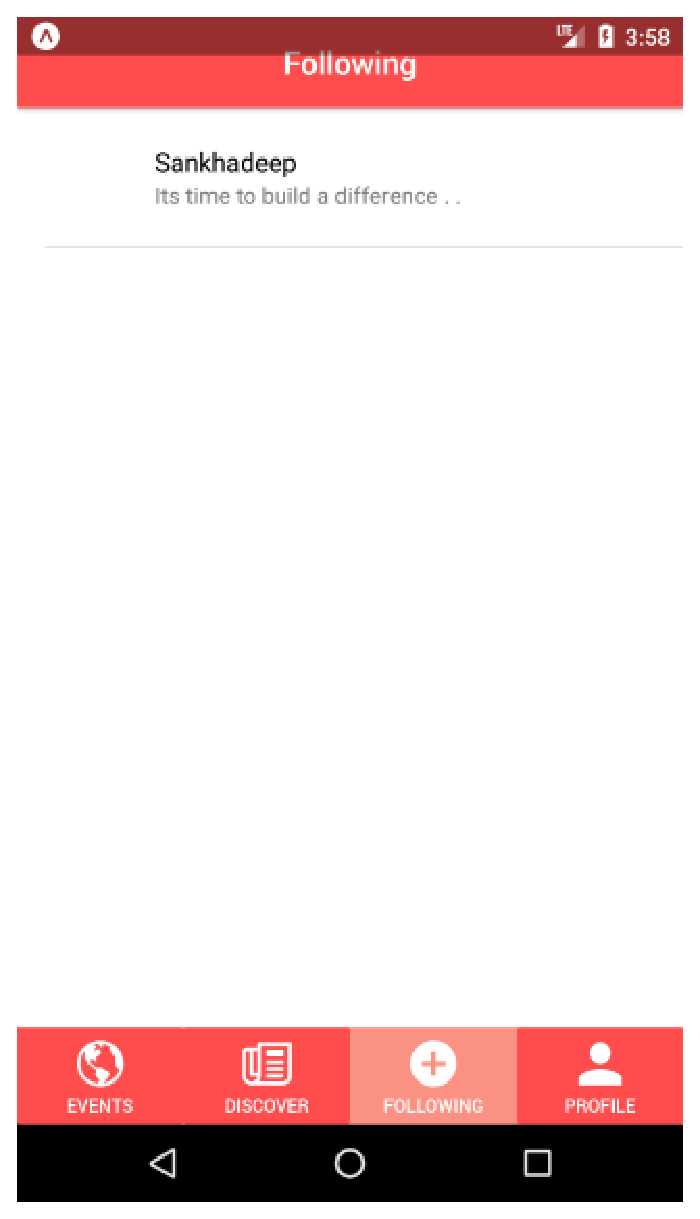
\includegraphics{Following_Screen.eps}
\newpage
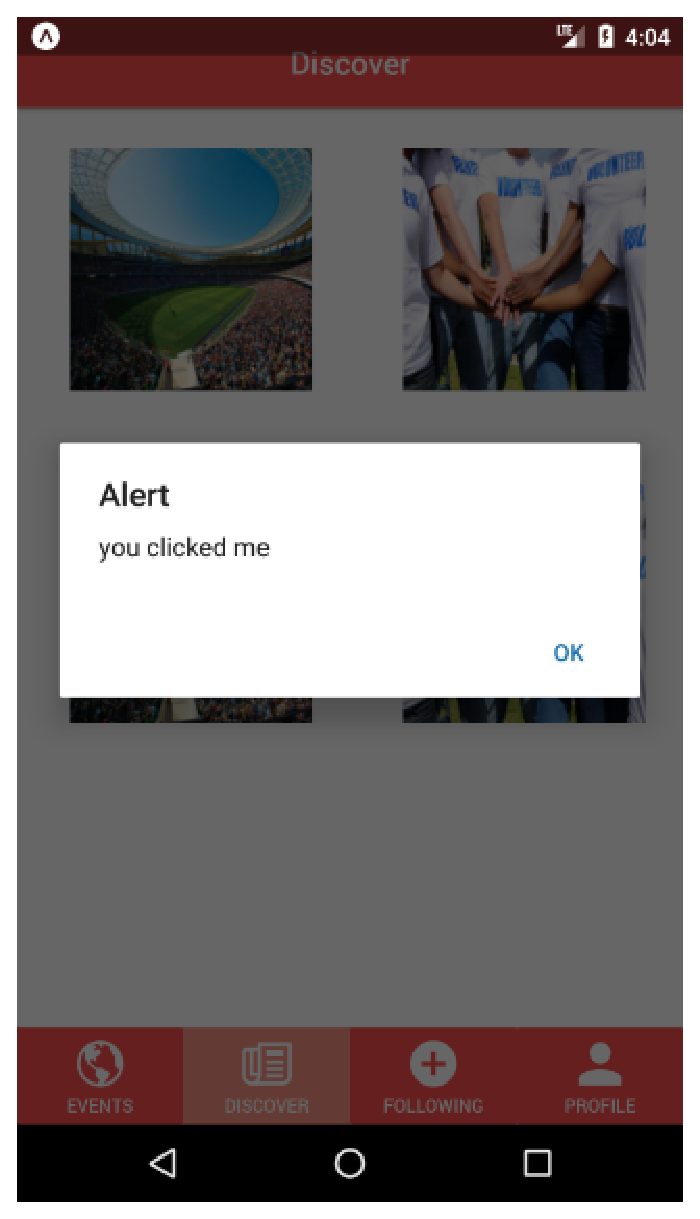
\includegraphics{Following_Screen_2.eps}


\end{document}
